\lstdefinestyle{mystyle}{
    breakatwhitespace=false,         
    breaklines=true,                 
    captionpos=b,                    
    keepspaces=true,                 
    numbers=left,                    
    numbersep=15pt,                  
    showspaces=false,                
    showstringspaces=false,
    showtabs=false,                  
    tabsize=2
}
 
\lstset{style=mystyle}

\section{OpenCV}\label{sec:opencv}
\paragraph{}
OpenCV (\url{https://opencv.org/}) is an open source computer vision library available under BSD licence. Its' alpha version was released in 1999 by an Intel Corporations' employee with hopes of a quicker and broader evolution of computer vision and artificial intelligence development. The library is primarily written in C and C++ and runs under any modern operating system. Apart from the core library, interfaces in other languages (such as Python, Java, etc.) are actively developed. Other major contributors to OpenCV include companies such as Google, Itseez and Arraiy.\cite{learning-opencv-3}
\paragraph{}
The library has been widely adopted both in business and in scientific research efforts. This popularity is a consequence of great computational efficiency that is achieved by optimized C++ code and the ability to make the most out of multicore processors. The liberal license also is a reason for it being so well-received. A commercial product can be freely built using OpenCV without any obligation to open-source it.
\paragraph{}
As computer vision goes hand-in-hand with machine learning, a fully-fledged ML module is also a part of OpenCV that is focused on clustering and statistical pattern recognition. This module mostly aims to be useful for computer vision tasks, but could also be used for solving other machine learning problems.
\paragraph{}
OpenCV since its' inception was developed to make computer vision infrastructure available to masses, to advance the research by providing core building blocks in order not to reinvent the wheel every single time. It also aimed to propagate the knowledge, standardize the development and advance vision-based applications. 

\section{OpenCV Python bindings}
\paragraph{}
Python is a general purpose programming language with rich standard library. It's main focus has always been both readability and clarity of the source code. It cooperates well with different programming paradigms, including object-oriented, imperative and, to a lesser degree, functional style. Python is a dynamic language that is often used for scripting purposes. It is slower in comparison to languages like C or C++ but can itself be easily extended with both of those. Simple Python wrappers can be applied to code written in C/C++ and this process allows to create highly efficient Python modules. Binding generators are used to create a bridge for the two languages. It would be tedious to write those wrapper functions by hand, that is why all of them are generated from the OpenCV C++ headers. 

\paragraph{}
Let us now see how easy it is to get started using OpenCV with Python bindings. The example below presents how to read an image and convert its' color space. It also shows how to save the effect of our work on the filesystem.

\begin{lstlisting}[language=Python, caption=Example usage of OpenCV with Python, basicstyle={\ttfamily}]
import cv2

# Let 'image_path' represent path to the image

# By default read as 8 bit per channel (no alpha channel)
image = cv2.imread(image_path)

# Alternatively can use one of the three flags
# IMREAD_COLOR, IMREAD_GRAYSCALE, IMREAD_UNCHANGED
grayscale = cv2.imread(image_path, cv2.IMREAD_GRAYSCALE)

# The color space can also be later changed
also_grayscale = cv2.cvtColor(image, cv2.COLOR_BGR2GRAY)

# Let the output path be somewhere on the filesystem
output_path = ...

# This is how a processed image can be saved on disk
cv2.imwrite(output_path, grayscale)
\end{lstlisting}

For more information regarding OpenCV usage please consult the official documentation available under: \url{https://docs.opencv.org/3.4.1/}.

\section{NumPy}
\paragraph{}
OpenCV Python bindings extensively use NumPy (\url{http://www.numpy.org/}). NumPy is a fundamental package for scientific computing and numerical operations with a MATLAB-like syntax. It's main object is the multidimensional array. It is a grid of values, all of the same type (often numbers), and indexed by a tuple of non-negative integers. Dimensions are called \textit{axes} and the number of axes defines the \textit{rank}.
\paragraph{}
\texttt{ndarray} (known also by the alias of \texttt{array}) is the array class in NumPy. It is important to remember that \texttt{numpy.array} is different from the class from Python's standard library (\texttt{array.array}). The latter one is designed for handling only one-dimensional arrays and its' functionality is also limited when compared to NumPy.

\paragraph{}
See how to make use of NumPy to create a histogram of values within some range and the most frequently occurring value.

\begin{lstlisting}[language=Python, caption=Example usage of NumPy, basicstyle={\ttfamily}]
# By convention a named import is used
import numpy as np

# Suppose 'angles' is an array of angles
# Let it be integers ranging 0 to 360

# Create the histogram
histogram, bin_edges = np.histogram(angles, bins=360, range=(0, 360))

# Select the most-frequent angle
the_angle = np.argmax(histogram)
\end{lstlisting}

\paragraph{}
For more information regarding NumPy usage please consult the official documentation available under: \url{https://docs.scipy.org/doc/}.

\section{Matplotlib}
\paragraph{}
Matplotlib (\url{https://matplotlib.org/}) is a 2D plotting library for Python. Plots, histograms, etc. can be achieved with just a few lines of code. The simple module that was used in this thesis is \texttt{pyplot}.

\begin{lstlisting}[language=Python, caption=Example usage of Matplotlib, label={lst:sinusoid}, basicstyle={\ttfamily}]
# Import just the pyplot module
from matplotlib import pyplot as plt

# NumPy proves to be very useful again
import numpy as np

# A list of values ranging from 0 to 40 with step 0.01
x = np.arange(0.0, 40.0, 0.01)
sin = np.sin(x)

figure, ax = plt.subplots()
ax.plot(x, sin)

# Label axes and add title for the plot
ax.set(
    xlabel='x',
    ylabel='sin(x)',
    title='This is a simple plot of sin function')
ax.grid()

# Save the plot to a file
figure.savefig("sin.png")

# Display the plot
plt.show()
\end{lstlisting}

Figure \ref{fig:matplotlib} shows the plot created by Matplotlib in combination with NumPy from code listing \ref{lst:sinusoid}.

\begin{figure}[H]
	\centering
	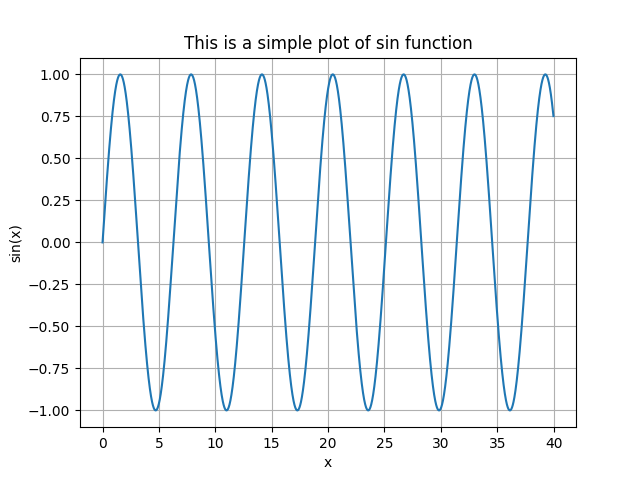
\includegraphics[width=\textwidth]{images/sin}
	\caption{Example plot from Matplotlib}
	\label{fig:matplotlib}
\end{figure}

\paragraph{}
For more information regarding Matplotlib usage please consult the official documentation available under: \url{https://matplotlib.org/2.2.2/contents.html}.